\documentclass[11pt, twoside, fleqn]{report}
\usepackage[backend=biber, style=ieee]{biblatex}
\usepackage[parfill, skip=1em]{parskip}
\usepackage[labelfont=bf]{caption}
\usepackage[margin=1in]{geometry}
\usepackage[hidelinks]{hyperref}
\usepackage{amssymb, booktabs, derivative, fancyhdr, float, graphicx, natex, pagecolor, pgfplots, siunitx, tikz}

% background and foreground colors
\definecolor{bgcolor}{HTML}{1e1e2e}
\definecolor{fgcolor}{HTML}{cdd6f4}

% catppuccin palette
\definecolor{p1}{HTML}{cba6f7}
\definecolor{p2}{HTML}{f38ba8}
\definecolor{p3}{HTML}{fab387}
\definecolor{p4}{HTML}{a6e3a1}
\definecolor{p5}{HTML}{89dceb}
\definecolor{p6}{HTML}{89b4fa}

% pagecolor
\pagecolor{bgcolor}
\color{fgcolor}

% biblatex
\addbibresource{references.bib}

% fancyhdr
\renewcommand{\chaptermark}[1]{\markboth{\thechapter\ #1}{}}
\renewcommand{\sectionmark}[1]{\markright{\thesection\ #1}}
\renewcommand{\footrulewidth}{0.4pt}

\fancypagestyle{mystyle}{
    \fancyfoot{}
    \fancyfoot[C]{\thepage}
}

% hyperref
\urlstyle{same}

% pgfplots
\pgfplotsset{compat=newest}

% custom
\newcommand{\dash}{\!\!-\!\!}
\newcommand{\state}[2]{\prescript{#1}{}{#2}}

\begin{document}

\pagestyle{empty}

\begin{titlepage}
    \null
    \vspace{\fill}
    \begin{center}
    \let \footnote \thanks
      {\LARGE \textbf{Simulation of Molecular Spectra} \par}
      {\large Theory and Applications}
      \vskip 1.5em
      {\large
        \lineskip .5em
        \begin{tabular}[t]{c}
          Nathan Phillips
        \end{tabular}\par}
      \vskip 1em
      {\large \today}
      \vskip 2em
    \end{center}
    \vspace{\fill}

    \begin{center}
        {\large{\textbf{Texas A\&M University}} \par}
        {\large{Department of Aerospace Engineering}}
    \end{center}
\end{titlepage}

\tableofcontents
\newpage
\listoffigures
\newpage
\listoftables
\newpage

\pagestyle{mystyle}

\chapter{Molecular Approximations}
\label{c:molecular_approximations}

\section{The Rigid Rotator}
\label{s:the_rigid_rotator}

\subsection{Theory}

The rigid rotator model assumes that the molecule is shaped like a dumbbell. Each of the two atoms of masses $m_1$ and $m_2$ is point-like and are affixed to one another via a massless rigid rod of radius $r$.

\begin{figure}[H]
    \centering
    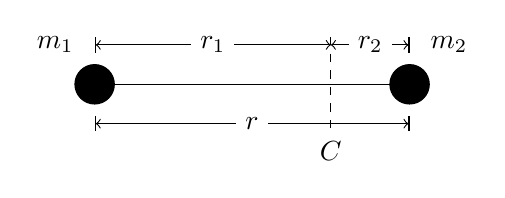
\begin{tikzpicture}
        \draw[fill=black](-2,0) circle(0.25);
        \node at (-2.5,0.5){$m_1$};
        \draw[color=black] (-2,0)rectangle(2,0);
        \draw[fill=black] (2,0)circle(0.25);
        \node at (2.5,0.5){$m_2$};

        \draw[|<->|](-2,-0.5)--(2,-0.5) node[midway, fill=white]{$r$};
        \draw[dashed](1,0.6)--(1,-0.6) node[below]{$C$};
        \draw[|<->](-2,0.5)--(1,0.5) node[midway, fill=white]{$r_1$};
        \draw[<->|](1,0.5)--(2,0.5) node[midway, fill=white]{$r_2$};
    \end{tikzpicture}
    \caption{Dumbbell model of a diatomic molecule.}
    \label{f:dumbbell_model}
\end{figure}

The classical expression for the rotational energy of a rigid body is
\begin{equation*}
    E = \frac{1}{2}I\omega^2,
\end{equation*}
where $\omega$ is the angular velocity and $I$ is the moment of inertia of the body about the axis of rotation $C$. For a point mass, the moment of inertia about an axis of a body is
\begin{equation*}
    I = \sum_i m_i r_i^2.
\end{equation*}
Using this definition, the magnitude of the angular momentum of the system can be found as
\begin{equation*}
    L = I\omega.
\end{equation*}
Using the angular momentum, the rotational energy of the system can now be expressed as
\begin{equation*}
    E = \frac{L^2}{2I}.
\end{equation*}

For the dumbbell model, the moment of inertia is
\begin{equation*}
    I = m_1r_1^2 + m_2r_2^2,
\end{equation*}
where
\begin{equation*}
    r_1 = \frac{m_2}{m_1 + m_2}r \quad\text{and}\quad r_2 = \frac{m_1}{m_1 + m_2}r
\end{equation*}
are the distances of the two masses $m_1$ and $m_2$ from the center of gravity $C$. Substituting these two expressions into the moment of inertia gives
\begin{equation*}
    I = \mu r^2,
\end{equation*}
where
\begin{equation*}
    \mu = \frac{m_1m_2}{m_1 + m_2}
\end{equation*}
is the reduced mass of the molecule.

\subsection{Energy Levels}

The appropriate Schr\"odinger Equation for the rigid rotator has $m = \mu$ and $V = 0$ since the model is regarded as perfectly rigid. Solving
\begin{equation*}
    \odv[2]{\psi}{x} + \pdv[2]{\psi}{y} + \pdv[2]{\psi}{z} + \frac{8\pi^2\mu}{h^2}E\psi = 0
\end{equation*}
leads to the energy eigenvalues given by
\begin{equation*}
    E = \frac{h^2J(J + 1)}{8\pi^2\mu r^2} = \frac{h^2J(J + 1)}{8\pi^2I},
\end{equation*}
where $J$ is the rotational quantum number. The quantized angular momentum can be found using the classical formula shown earlier, which leads to
\begin{equation*}
    L = \sqrt{2EI} = \frac{h}{2\pi}\sqrt{J(J + 1)}.
\end{equation*}
The angular velocity $\omega$ and rotational frequency $\nu\_{rot}$ can also be found as
\begin{equation*}
    \omega = \frac{h}{2\pi I}\sqrt{J(J + 1)} \quad\text{and}\quad \nu\_{rot} = \frac{\omega}{2\pi} = \frac{h}{4\pi^2I}\sqrt{J(J + 1)}.
\end{equation*}

\subsection{Spectrum}

The emission of a light quantum results from the transition of the rotator from a higher to a lower energy level. Conversely, the absorption of a light quantum produces a transition from a lower to a higher level. The wave number $\nu$ of the emitted or absorbed quantum is
\begin{equation*}
    \nu = \frac{E'}{hc} - \frac{E''}{hc}.
\end{equation*}
The single prime $'$ refers to the upper state, while the double prime $''$ refers to the lower state.

The quantity $E/hc$ is called the rotational term value and is denoted $F(J)$. The value of $F(J)$ is given as
\begin{equation*}
    F(J) = \frac{E}{hc} = \frac{h}{8\pi^2cI}J(J + 1) = BJ(J + 1).
\end{equation*}
The constant
\begin{equation*}
    B = \frac{h}{8\pi^2cI}
\end{equation*}
is called the rotational constant and is essentially the reciprocal moment of inertia. These two definitions allow for the rewriting of the wavenumber as
\begin{equation*}
    \nu = F(J')- F(J'') = BJ'(J' + 1) - BJ''(J'' + 1).
\end{equation*}

To find which frequencies are actually emitted or absorbed, selection rules for the rotational quantum number $J$ must be established. The selection rule for $J$ is
\begin{equation*}
    J' = J'' \pm 1; \quad\text{that is,}\quad \Delta{}J = J' - J'' = \pm 1.
\end{equation*}

Because $J' > J''$ always (due to $J'$ being the upper state), only $\Delta{}J = +1$ needs to be considered. Therefore, the absorbed or emitted lines of the rigid rotator are given by
\begin{equation*}
    \nu = F(J'' + 1) - F(J'') = B(J'' + 1)(J'' + 2) - BJ''(J'' + 1) = 2B(J'' + 1).
\end{equation*}
Writing $J$ instead of $J''$ when only the $J$ value of the lower state occurs, we get
\begin{equation*}
    \nu = 2B(J + 1) \quad\text{for}\quad J = 0, 1, 2, \dotsb.
\end{equation*}
The rotational frequency of the rigid rotator is
\begin{equation*}
    \nu\_{rot} = 2cB\sqrt{J(J + 1)}.
\end{equation*}

\section{The Harmonic Oscillator}
\label{s:the_harmonic_oscillator}

\subsection{Theory}

In classical mechanics, the equation of motion for a simple harmonic oscillator is
\begin{equation*}
    F = -kx = m\odv[2]{x}{t},
\end{equation*}
where $F$ is the force experienced by the particle toward the equilibrium position which is proportional to the distance $x$ away from the equilibrium position. Solving the differential equation for $x$ yields
\begin{equation*}
    x = x_0\sin(2\pi t\nu\_{vib} + \varphi),
\end{equation*}
where the vibrational frequency $\nu\_{vib}$ is given by
\begin{equation*}
    \nu\_{vib} = \frac{1}{2\pi}\sqrt{\frac{k}{m}}.
\end{equation*}

The potential energy for a linear spring is
\begin{equation*}
    V = \frac{1}{2}kx^2 = 2\pi^2mx^2\nu\_{vib}^2
\end{equation*}

The restoring force exerted by the two atoms in a molecule after being displaced from their equilibrium position $r_e$ can be modeled by the equation of motion for a spring as
\begin{equation*}
    m_1\odv[2]{r_1}{t} = -k(r - r_e)
\end{equation*}
and
\begin{equation*}
    m_2\odv[2]{r_2}{t} = -k(r - r_e).
\end{equation*}
Substituting $r$ in place of both $r_1$ and $r_2$ gives the single equation
\begin{equation*}
    \frac{m_1m_2}{m_1 + m_2}\odv[2]{r}{t} = -k(r - r_e),
\end{equation*}
which is equivalent to
\begin{equation*}
    \mu\odv[2]{(r - r_e)}{t} = -k(r - r_e)
\end{equation*}
since $r_e$ is constant. From direct comparison with the classical equation of motion for a harmonic oscillator, it follows that the vibrational frequency of the molecule is
\begin{equation*}
    \nu\_{vib} = \frac{1}{2\pi}\sqrt{\frac{k}{\mu}}.
\end{equation*}

\subsection{Energy Levels}

The Schr\"odinger equation for the harmonic oscillator is
\begin{equation*}
    \odv[2]{\psi}{x} + \frac{8\pi^2\mu}{h^2}\pr*{E - \tfrac{1}{2}kx^2}\psi = 0.
\end{equation*}
Solving this equation leads to the energy eigenvalues given by
\begin{equation*}
    E(v) = \frac{h}{2\pi}\sqrt{\frac{k}{\mu}}\pr*{v + \tfrac{1}{2}} = h\nu\_{vib}\pr*{v + \tfrac{1}{2}} \quad\text{for}\quad v = 0, 1, 2, \dotsb.
\end{equation*}
Rewriting the energy as the vibrational term value $G(v)$ gives
\begin{equation*}
    G(v) = \frac{E(v)}{hc} = \frac{\nu\_{vib}}{c}\pr*{v + \tfrac{1}{2}} = \omega\pr*{v + \tfrac{1}{2}},
\end{equation*}
where the quantity $\nu\_{vib}/c$ is designated $\omega$ and measured in \unit{cm^{-1}}.

\subsection{Spectrum}

Similarly to the rigid rotor, the wavenumber of the emitted or absorbed light is given by
\begin{equation*}
    \nu = \frac{E(v')}{hc} - \frac{E(v'')}{hc} = G(v') - G(v''),
\end{equation*}
where $v'$ and $v''$ are the quantum numbers of the upper and lower state, respectively.

The selection rule for the vibrational quantum number of the harmonic oscillator is
\begin{equation*}
    \Delta{}v = v' - v'' = \pm 1.
\end{equation*}
Again denoting $J''$ as $J$, the wavenumber of the emitted or absorbed light is
\begin{equation*}
    \nu = G(v + 1) - G(v) = \omega.
\end{equation*}

\section{The Anharmonic Oscillator}
\label{s:the_anharmonic_oscillator}

\subsection{Theory}

A first approximation to the actual potential energy function of the molecule can be written as
\begin{equation*}
    U = f(r - r_e)^2 - g(r - r_e)^3,
\end{equation*}
where $f$ and $g$ are coefficients, with $g$ being much smaller than $f$. Better approximations can be made by adding higher order terms to this expression.

The motion of the anharmonic oscillator can be represented as a superposition of fundamental and overtone vibrations as the following Fourier series:
\begin{equation*}
    x = x_{01}\sin{2\pi\nu\_{vib}t} + x_{02}(3 + \cos{2\pi2\nu\_{vib}t}) + x_{03}\sin{2\pi3\nu\_{vib}t} + \dotsb.
\end{equation*}
In this expression, $x_{01}$, $x_{02}$, and $x_{03}$ are the amplitudes of the fundamental, the first, and the second overtone, respectively. If the anharmonicity is small $(g \ll f)$, then $x_{02} \ll x_{01}$ and $x_{03} \ll x_{02}$. However, $x_{02}$ and $x_{03}$ are proportional to the square and cube of $x_{01}$, respectively and rapidly become more important as $x_{01}$ increases. Because of the asymmetric potential curve, the time average of the position is not at $x = 0$, but instead at $x = 3x_{02}$.

The frequency of the vibrations is given as
\begin{equation*}
    \nu\_{vib} = \frac{1}{2\pi}\sqrt{\frac{k}{\mu}}
\end{equation*}
for very small amplitudes only. This factor decreases slowly as the amplitude $x_{01}$ increases.

\subsection{Energy Levels}

Substituting the anharmonic potential energy function into the Schr\"odinger equation and solving for the energy eigenvalues gives
\begin{equation*}
    E_v = hc\omega_e\pr*{v + \tfrac{1}{2}} - hc\omega_ex_e\pr*{v + \tfrac{1}{2}}^2 + hc\omega_ey_e\pr*{v + \tfrac{1}{2}}^3 + \dotsb.
\end{equation*}
Written as the vibrational term $G(v)$, this becomes
\begin{equation*}
    G(v) = \omega_e\pr*{v + \tfrac{1}{2}} - \omega_ex_e\pr*{v + \tfrac{1}{2}}^2 + \omega_ey_e\pr*{v + \tfrac{1}{2}}^3 + \dotsb,
\end{equation*}
where $v$ is the vibrational quantum number, $\omega_ex_e \ll \omega_e$, and $\omega_ey_e \ll \omega_ex_e$. This equation directly shows that the energy levels of the anharmonic oscillator are not equidistant like those of the harmonic oscillator.

The zero-point energy of the anharmonic oscillator is given by setting $v = 0$ in the vibrational term above:
\begin{equation*}
    G(0) = \tfrac{1}{2}\omega_e - \tfrac{1}{2}\omega_ex_e + \tfrac{1}{8}\omega_ey_e + \dotsb.
\end{equation*}

\subsection{Spectrum}

The selection rule for the anharmonic oscillator is given by
\begin{equation*}
    \Delta{}v = \pm 1
\end{equation*}
for the most intense transitions, but the two selection rules of
\begin{equation*}
    \Delta{}v = \pm 2 \quad\text{and}\quad \Delta{}v = \pm 3
\end{equation*}
can also appear with decreasing intensity.

The formula for the series of absorption bands $1\dash0$, $2\dash0$, $3\dash0$, $\dotsb$ is given as
\begin{equation*}
    \nu\_{abs} = G(v') - G(0) = G_0(v') = \omega_0v' - \omega_0x_0v'^2 + \omega_0y_0v'^3 + \dotsb.
\end{equation*}

\section{The Nonrigid Rotator}
\label{s:the_nonrigid_rotator}

\subsection{Energy Levels}

A good approximation shows that the rotational terms of the nonrigid rotator are given by
\begin{equation*}
    F(J) = \frac{E_r}{hc} = B[1 - uJ(J + 1)]J(J + 1),
\end{equation*}
where the value $B[1 - uJ(J + 1)]$ now appears in the place of $B$ in the equation for the rigid rotator. This equation can also be written as
\begin{equation*}
    F(J) = BJ(J + 1) - DJ^2(J + 1)^2,
\end{equation*}
where $D$ always has a positive value with this choice of sign. If cubic and higher powers in the potential energy are included, the rotational terms values are
\begin{equation*}
    F(J) = BJ(J + 1) - DJ^2(J + 1)^2 + HJ^3(J + 1)^3 + \dotsb.
\end{equation*}

\subsection{Spectrum}

The selection rule for the infrared spectrum of the rigid rotator $\Delta{}J = \pm 1$ is also valid for the nonrigid rotator. Therefore, the wavenumbers of the lines of the infrared rotation spectrum are
\begin{equation*}
    \nu = F(J + 1) - F(J) = 2B(J + 1) - 4D(J + 1)^3.
\end{equation*}

\section{The Vibrating Rotator}
\label{s:the_vibrating_rotator}

\subsection{Energy Levels}

Since the molecule is vibrating, the internuclear distance and therefore the moment of inertia and the rotational constant $B$ are changing rapidly. Since the period of vibration is small compared to the period of rotation, the mean value of $B$ is
\begin{equation*}
    B_v = \frac{h}{8\pi^2c\mu}\bk*{\bar{\frac{1}{r^2}}},
\end{equation*}
where $\overline{1/r^2}$ is the mean value of $1/r^2$ during the vibration. The value of $B_v$ will be expected to be smaller than the equilibrium constant $B_e$ since the mean nuclear separation will be greater. The value of $B_e$ is given by
\begin{equation*}
    B_e = \frac{h}{8\pi^2c\mu{}r_e^2} = \frac{h}{8\pi^2cI_e}.
\end{equation*}
To a first approximation, the rotational constant $B_v$ in the vibrational state $v$ is given as
\begin{equation*}
    B_v = B_e - \alpha_e\pr*{v + \tfrac{1}{2}} + \dotsb,
\end{equation*}
where $\alpha_e$ is a constant which is small compared to $B_e$. The ratio $\alpha_e/B_e$ is only slightly larger than $\omega_ex_e/\omega_e$.

A mean rotational constant $D_v$ representing the contribution of centrifugal force can be found as
\begin{equation*}
    D_v = D_e + \beta_e\pr*{v + \tfrac{1}{2}} + \dotsb.
\end{equation*}
In this equation, $\beta_e$ is small compared to
\begin{equation*}
    D_e = \frac{4B_e^3}{\omega_e^2}.
\end{equation*}

The rotational terms in a given vibrational level are therefore given by
\begin{equation*}
    F_v(J) = B_vJ(J + 1) - D_vJ^2(J + 1)^2 + \dotsb.
\end{equation*}
Taking into account the interaction between vibration and rotation, the term values for the vibrating rotator are
\begin{equation*}
    T = G(v) + F_v(J) = \omega_e\pr*{v + \tfrac{1}{2}} - \omega_ex_e\pr*{v + \tfrac{1}{2}}^2 + \dotsb + B_vJ(J + 1) - D_vJ^2(J + 1)^2 + \dotsb.
\end{equation*}
For the lowest vibrational state $v = 0$, the rotational constant $B_0$ must be used in this equation.

If very precise measurements are available, higher powers of $\pr*{v + \tfrac{1}{2}}$ can be taken into account using
\begin{equation*}
    B_v = B_e - \alpha_e\pr*{v + \tfrac{1}{2}} + \gamma_e\pr*{v + \tfrac{1}{2}}^2 + \dotsb.
\end{equation*}
In higher powers of $J(J + 1)$, the rotational term can be expressed as
\begin{equation*}
    F_v(J) = B_vJ(J + 1) - D_vJ^2(J + 1)^2 + H_vJ^3(J + 1)^3 + \dotsb,
\end{equation*}
where the rotational constant $H_v$ is given as
\begin{equation*}
    H_v \approx H_e = \frac{2D_e}{3\omega_e^2}(12B_e^2 - \alpha_e\omega_e)
\end{equation*}
to a first approximation.

\section{The Symmetric Top}
\label{s:the_symmetric_top}

\subsection{Theory}

\subsection{Energy Levels}

\subsection{Spectra}


\chapter{Structure of Electronic Transitions}
\label{c:structure_of_electronic_transitions}

\section{Total Energy}
\label{s:total_energy}

The total energy $E$ of a molecule is approximated by
\begin{equation*}
    E = E_e + E_v + E_r,
\end{equation*}
that is, the sum of the electronic, vibrational, and rotational energy terms. The same equation written in wavenumber units is
\begin{equation}
    T = T_e + G + F.
\end{equation}

\section{Vibrational Term}
\label{s:vibrational_term}

For the vibrational and rotational states of the molecule in different electronic states, the vibrating rotator model is used \cite{herzberg:diatomic}. The fourth-order approximation for the vibrational term $G(v)$ is
\begin{equation}
    G(v) = \omega_e\pr*{v + \tfrac{1}{2}} - \omega_ex_e\pr*{v + \tfrac{1}{2}}^2 + \omega_ey_e\pr*{v + \tfrac{1}{2}}^3 + \omega_ez_e\pr*{v + \tfrac{1}{2}}^4 + \dotsb.
\end{equation}

\section{Rotational Term}
\label{s:rotational_term}

The rotational term $F_v(J)$ approximated to the third order is given as
\begin{equation}
    F_v(J) = B_vJ(J + 1) - D_vJ^2(J + 1)^2 + H_vJ^3(J + 1)^3 + \dotsb.
\end{equation}
The rotational constant $B_v$ can be approximated to the third order as (Herz. pp. 108)
\begin{equation*}
    B_v = B_e - \alpha_e\pr*{v + \tfrac{1}{2}} + \gamma_e\pr*{v + \tfrac{1}{2}}^2 + \delta_e\pr*{v + \tfrac{1}{2}}^3 + \dotsb.
\end{equation*}
The centrifugal distortion constant $D_v$ can be approximated to the first order as (Herz. pp. 107)
\begin{equation}
    D_v = D_e + \beta_e\pr*{v + \tfrac{1}{2}} + \dotsb.
\end{equation}
Finally, the third-order constant $H_v$ can be found as the first approximation (Herz. pp. 109)
\begin{equation}
    H_v \approx H_e.
\end{equation}

\section{Transition Wavenumbers}
\label{s:transition_wavenumbers}

The wavenumbers of the spectral lines corresponding to the transitions between two electronic states (in emission or absorption) are given by
\begin{equation}
    \nu = T' - T'' = (T_e' - T_e'') + (G' - G'') + (F' - F'').
\end{equation}
That is, the emitted or absorbed frequencies can be expressed as sums of their constituent parts:
\begin{equation*}
    \nu = \nu_e + \nu_v + \nu_r.
\end{equation*}


\chapter{Intensities in Rotation-Vibration Spectra}
\label{c:intensities_in_rotation-vibration_spectra}

\section{Vibration}
\label{s:vibration}

\subsection{Partition Function}

The quantities given by
\begin{equation*}
    \eul^{-G_0(v)hc/kT}
\end{equation*}
give the relative numbers of molecules in the different vibrational levels relative to the number of molecules in the lowest vibrational level. A more useful equation gives the ratio between the number of molecules in a certain vibrational level relative to the total number of molecules as
\begin{equation*}
    \frac{N_v}{N} = \frac{\eul^{-G_0(v)hc/kT}}{Q_v}.
\end{equation*}
Here, $Q_v$ is the vibrational partition function and is given by
\begin{equation*}
    Q_v = \sum_{v=0}^{\infty}\eul^{-G_0(v)hc/kT} = 1 + \eul^{-G_0(1)hc/kT} + \eul^{-G_0(2)hc/kT} + \dotsb.
\end{equation*}

\subsection{Intensities}

\subsection{Franck-Condon Factors}

\section{Rotation}
\label{s:rotation}

\subsection{Partition Function}

The number of molecules $N_J$ in the rotational level $J$ of the lowest vibrational state at the temperature $T$ is proportional to
\begin{equation*}
    (2J + 1)\eul^{-F(J)hc/kT}.
\end{equation*}
For most practical cases like a rigid rotator with $\Lambda = 0$,
\begin{equation*}
    N_J \propto (2J + 1)\eul^{-BJ(J + 1)hc/kT}.
\end{equation*}
The number of molecules in the different rotational states does not increase linearly and goes through a maximum with the rotational quantum number
\begin{equation*}
    J\_{max} = \sqrt{\frac{kT}{2Bhc}} - \frac{1}{2}.
\end{equation*}

The ratio of the actual number of molecules in a given rotational state is given by
\begin{equation*}
    \frac{N_J}{N} = (2J + 1)\frac{\eul^{-F(J)hc/kT}}{Q_r},
\end{equation*}
where the rotational partition function $Q_r$ is given as
\begin{equation}
    Q_r = \sum_{J=0}^{\infty}(2J + 1)\eul^{-F(J)hc/kT} = 1 + 3\eul^{-F(1)hc/kT} + 5\eul^{-F(2)hc/kT} + \dotsb.
\end{equation}

For higher vibrational levels,
\begin{equation}
    N_J \propto (2J + 1)\eul^{-(G + F)hc/kT}.
\end{equation}
However, the factor $\eul^{-Ghc/kT}$ can be separated off since the distribution over the rotational levels is the same but the absolute population of all the levels is considerably smaller than for the lowest vibrational level.

\subsection{Intensities}

\subsection{H\"onl-London Factors}

\begin{table}[H]
    \centering
    \caption{H\"onl-London factors \cite{herzberg:diatomic}.}
    \label{t:honl-london_factors}
    \begin{tabular}{ccc}
        \toprule
        Branch & Absorption & Emission \\
        \midrule
        \multicolumn{3}{c}{$\adif{\Lambda} = 0$ \textit{Transitions}} \\
        \cmidrule(lr){1-3}
        $S_J^R$ & $\dfrac{(J'' + 1 + \Lambda'')(J'' + 1 - \Lambda'')}{J'' + 1}$ & $\dfrac{(J' + \Lambda')(J' - \Lambda')}{J'}$ \\
        \addlinespace[0.5em]
        $S_J^Q$ & $\dfrac{(2J'' + 1)\Lambda''^2}{J''(J'' + 1)}$ & $\dfrac{(2J' + 1)\Lambda'^2}{J'(J' + 1)}$ \\
        \addlinespace[0.5em]
        $S_J^P$ & $\dfrac{(J'' + \Lambda'')(J'' - \Lambda'')}{J''}$ & $\dfrac{(J' + 1 + \Lambda')(J' + 1 - \Lambda')}{J' + 1}$ \\
        \addlinespace[0.5em]
        \multicolumn{3}{c}{$\adif{\Lambda} = +1$ \textit{Transitions}} \\
        \cmidrule(lr){1-3}
        $S_J^R$ & $\dfrac{(J'' + 2 + \Lambda'')(J'' + 1 + \Lambda'')}{4(J'' + 1)}$ & $\dfrac{(J' + \Lambda')(J' - 1 + \Lambda')}{4J'}$ \\
        \addlinespace[0.5em]
        $S_J^Q$ & $\dfrac{(J'' + 1 + \Lambda'')(J'' - \Lambda'')(2J'' + 1)}{4J''(J'' + 1)}$ & $\dfrac{(J' + \Lambda')(J' + 1 - \Lambda')(2J' + 1)}{4J'(J' + 1)}$ \\
        \addlinespace[0.5em]
        $S_J^P$ & $\dfrac{(J'' - 1 - \Lambda'')(J'' - \Lambda'')}{4J''}$ & $\dfrac{(J' + 1 - \Lambda')(J' + 2 - \Lambda')}{4(J' + 1)}$ \\
        \addlinespace[0.5em]
        \multicolumn{3}{c}{$\adif{\Lambda} = -1$ \textit{Transitions}} \\
        \cmidrule(lr){1-3}
        $S_J^R$ & $\dfrac{(J'' + 2 - \Lambda'')(J'' + 1 - \Lambda'')}{4(J'' + 1)}$ & $\dfrac{(J' - \Lambda')(J' - 1 - \Lambda')}{4J'}$ \\
        \addlinespace[0.5em]
        $S_J^Q$ & $\dfrac{(J'' + 1 - \Lambda'')(J'' + \Lambda'')(2J'' + 1)}{4J''(J'' + 1)}$ & $\dfrac{(J' - \Lambda')(J' + 1 + \Lambda')(2J' + 1)}{4J'(J' + 1)}$ \\
        \addlinespace[0.5em]
        $S_J^P$ & $\dfrac{(J'' - 1 + \Lambda'')(J'' + \Lambda'')}{4J''}$ & $\dfrac{(J' + 1 + \Lambda')(J' + 2 + \Lambda')}{4(J' + 1)}$ \\
        \bottomrule
    \end{tabular}
\end{table}

\section{Band Intensity}
\label{s:band_intensity}

The variation of the intensity of the lines in a rotation-vibration band as a function of $J$ is essentially given by the thermal distribution of the rotational levels. In this approximation, it is assumed that the transition probability is the same for all lines of a band. In reality, there is a slight dependence on $J$ and $\Delta{}J$. For the case of $\Lambda = 0$ when only the $P$ and $R$ branches appear, $J' + J'' + 1$ can be used in place of $2J + 1$; that is, the intensity depends on the mean value of $2J + 1$ for the upper and lower states. The $J$ value of the initial state should be used in the exponential term. For absorption, that is $J''$; for emission, $J'$.

The intensities of the lines of rotation or rotation-vibration bands in absorption are
\begin{equation}
    I\_{abs} = \frac{C\_{abs}\nu}{Q_r}(J' + J'' + 1)\eul^{-F(J'')hc/kT}.
\end{equation}
In emission, they are
\begin{equation}
    I\_{em} = \frac{C\_{em}\nu^4}{Q_r}(J' + J'' + 1)\eul^{-F(J')hc/kT}.
\end{equation}


\chapter{Quantum Numbers}
\label{c:quantum_numbers}

\section{Atoms}
\label{s:atoms}

\subsection{Atomic Term Symbol}

\begin{equation*}
    \state{2S + 1}{L_{J}}
\end{equation*}

\section{Molecules}
\label{s:molecules}

\subsection{Molecular Term Symbol}

\begin{equation*}
    \state{2S + 1}{\Lambda_{\Omega, (g/u)}^{(+/-)}}
\end{equation*}


\chapter{Hund's Coupling Cases}
\label{c:hunds_coupling_cases}

\section{Hund's Case (a)}
\label{s:hunds_case_a}

\subsection{Good Quantum Numbers}

\begin{equation*}
    \Lambda, S, \Sigma, J, \Omega
\end{equation*}

\subsection{Selection Rules}

General rules
\begin{align*}
    g        & \nleftrightarrow g, \quad g \leftrightarrow u, \quad u \nleftrightarrow u \\
    \adif{J} & = 0, \pm 1 \text{ with the restriction } J = 0 \nrightarrow J = 0
\end{align*}

Rules common to both (a) and (b)
\begin{align*}
    \adif{\Lambda} & = 0, \pm 1 \\
    \adif{S}       & = 0
\end{align*}

Rules for case (a) only
\begin{align*}
    \adif{\Sigma} & = 0                                                             \\
    \adif{\Omega} & = 0, \pm 1                                                      \\
    \adif{J}      & = 0 \text{ is forbidden for } \Omega = 0 \rightarrow \Omega = 0
\end{align*}

\subsection{Term Values}

\begin{equation*}
    F_{v}(J) = B_{v}[J(J + 1) - \Omega^{2}]
\end{equation*}

\section{Hund's Case (b)}
\label{s:hunds_case_b}

\subsection{Good Quantum Numbers}

\begin{equation*}
    \Lambda, N, S, J
\end{equation*}

\subsection{Selection Rules}

General rules
\begin{align*}
    g        & \nleftrightarrow g, \quad g \leftrightarrow u, \quad u \nleftrightarrow u \\
    \adif{J} & = 0, \pm 1 \text{ with the restriction } J = 0 \nrightarrow J = 0
\end{align*}

Rules common to both (a) and (b)
\begin{align*}
    \adif{\Lambda} & = 0, \pm 1 \\
    \adif{S}       & = 0
\end{align*}

Rules for case (b) only
\begin{align*}
    \adif{N} & = 0, \pm 1                                                          \\
    \adif{N} & = 0 \text{ is forbidden for } \Sigma\dash\Sigma \text{ transitions}
\end{align*}

\subsection{Term Values}

$\state{2}{\Sigma}$ states
\begin{align*}
    F_{1}(N) & = B_{v}N(N + 1) + \tfrac{1}{2}\gamma N      \\
    F_{2}(N) & = B_{v}N(N + 1) - \tfrac{1}{2}\gamma(N + 1)
\end{align*}

$\state{3}{\Sigma}$ states
\begin{align*}
    F_{1}(N) & = B_{v}N(N + 1) + (2N + 3)B_{v} - \lambda - \sqrt{(2N + 3)^{2}B_{v}^{2} + \lambda^{2} - 2\lambda B_{v}} + \gamma(N + 1) \\
    F_{2}(N) & = B_{v}N(N + 1)                                                                                                         \\
    F_{3}(N) & = B_{v}N(N + 1) - (2N - 1)B_{v} - \lambda + \sqrt{(2N - 1)^{2}B_{v}^{2} + \lambda^{2} - 2\lambda B_{v}} - \gamma N
\end{align*}


\chapter{Uncoupling}
\label{c:uncoupling}

\section{\texorpdfstring{$\Lambda$}{Λ} Doubling}
\label{s:lambda_doubling}

\section{Spin Uncoupling}
\label{s:spin_uncoupling}

\subsection{Doublet States}

\begin{align*}
    F_{1}(J) & = B_{v}\ab[\ab(J + \tfrac{1}{2})^{2} - \Lambda^{2} - \tfrac{1}{2}\sqrt{4\ab(J + \tfrac{1}{2})^{2} + Y(Y - 4)\Lambda^{2}}] - D_{v}J^{4}       \\
    F_{2}(J) & = B_{v}\ab[\ab(J + \tfrac{1}{2})^{2} + \Lambda^{2} - \tfrac{1}{2}\sqrt{4\ab(J + \tfrac{1}{2})^{2} + Y(Y - 4)\Lambda^{2}}] - D_{v}(J + 1)^{4}
\end{align*}

\subsection{Triplet States}

\begin{align*}
    F_{1}(J) & = B_{v}\ab[J(J + 1) - \sqrt{Z_{1}} - 2Z_{2}] - D_{v}\ab(J - \tfrac{1}{2})^{4} \\
    F_{2}(J) & = B_{v}[J(J + 1) + 4Z_{2}] - D_{v}\ab(J + \tfrac{1}{2})^{4}                   \\
    F_{3}(J) & = B_{v}\ab[J(J + 1) + \sqrt{Z_{1}} - 2Z_{2}] - D_{v}\ab(J + \tfrac{3}{2})^{4}
\end{align*}
where
\begin{align*}
    Z_{1} & = \Lambda^{2}Y(Y - 4) + \tfrac{4}{3} + 4J(J + 1)                      \\
    Z_{2} & = \frac{1}{3Z_{1}}\ab[\Lambda^{3}Y(Y - 1) - \tfrac{4}{9} - 2J(J + 1)]
\end{align*}


\chapter{Electronic Transitions}
\label{c:electronic_transitions}

\section{\texorpdfstring{$\state{3}{\Sigma}\dash\state{3}{\Sigma}$}{3Σ-3Σ} Transitions}
\label{s:3_sigma_to_3_sigma_transitions}

\section{\texorpdfstring{$\state{2}{\Pi}\dash\state{2}{\Pi}$}{2Π-2Π} Transitions}
\label{s:2_pi_to_2_pi_transitions}


\chapter{Laser-Induced Fluorescence}
\label{c:laser-induced_fluorescence}

Laser-induced fluorescence is a method of spectroscopy that excites a molecule into a higher electronic state via the absorption of laser radiation. A single ro-vibrational band is isolated and excited. Next, the molecule relaxes back into the original electronics state, filling multiple lower vibrational states in the process. These vibrational states are filled according to the known Franck-Condon factors.

Figure \ref{f:laser-induced_fluorescence_in_iodine} below shows the jump from the ground state to the excited state via laser excitation. Subsequently, the molecule relaxes to fill multiple vibrational states within the original electronic state.

\begin{figure}[H]
    \centering
    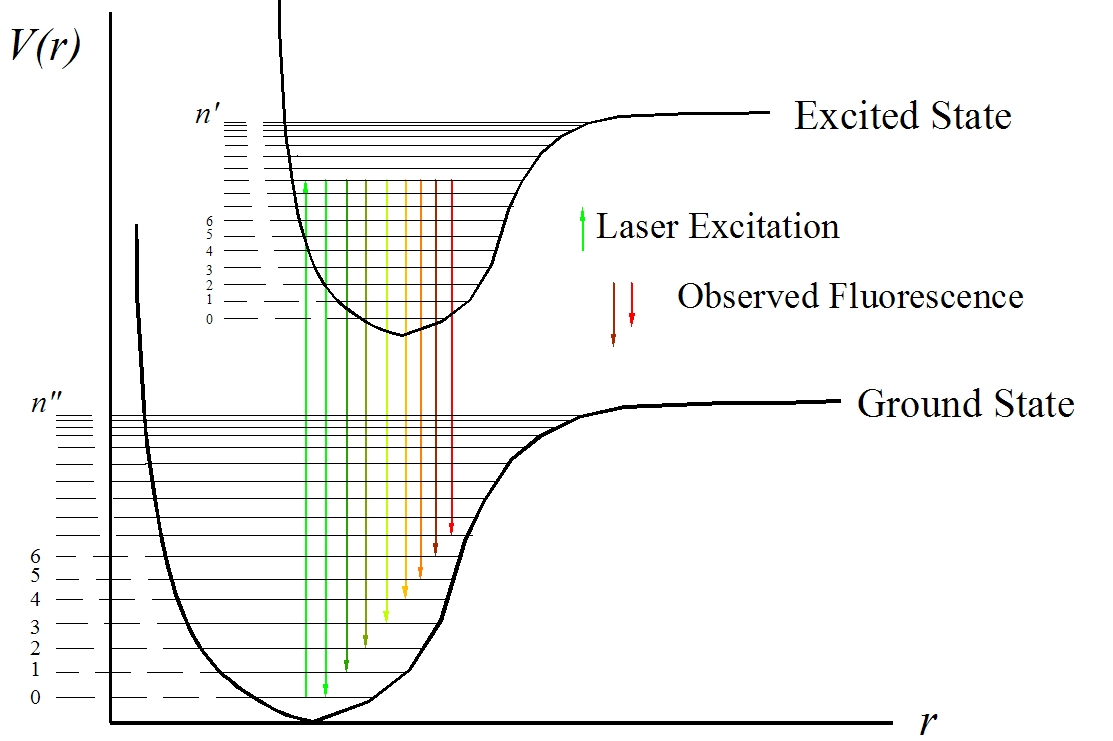
\includegraphics[width=0.8\textwidth]{img/lif_bands}
    \caption{Laser-induced fluorescence in Iodine.}
    \label{f:laser-induced_fluorescence_in_iodine}
\end{figure}


\chapter{Spectral Lineshapes}
\label{c:spectral_lineshapes}

\section{Gaussian Profile}
\label{s:gaussian_profile}

The probability density function (PDF) for the Gaussian profile is
\begin{equation*}
    G(x; x_0, \sigma) = \frac{1}{\sigma\sqrt{2\pi}}\exp\pr*{-\frac{(x - x_0)^2}{2\sigma^2}},
\end{equation*}
where $x$ is the desired wavenumber, $x_0$ is the intensity at a wavenumber peak, and $\sigma$ is the broadening parameter.

\section{Lorentzian Profile}
\label{s:lorentzian_profile}

The PDF for the Lorentzian profile is
\begin{equation*}
    L(x; x_0, \gamma) = \frac{1}{\pi}\bk*{\frac{\gamma}{(x - x_0)^2 + \gamma^2}},
\end{equation*}
where $\gamma$ is the broadening parameter.

\section{Voigt Profile}
\label{s:voigt_profile}

The Voigt profile is a convolution of the Gaussian and Lorentzian profiles. The PDF for the Voigt profile is
\begin{equation*}
    V(x; x_0, \sigma, \gamma) = \frac{1}{\sigma\sqrt{2\pi}}\Re[w(z)],
\end{equation*}
where
\begin{equation*}
    w(z) \defn \eul^{-z^2}\erfc(-\img z) = \eul^{-z^2}\pr*{1 + 
    \frac{2\img}{\sqrt{\pi}}\int_0^z \eul^{t^2} \odif{t}},
\end{equation*}
and
\begin{equation*}
    z = \frac{(x - x_0) + \img\gamma}{\sigma\sqrt{2}}.
\end{equation*}

\begin{figure}[H]
    \centering
    \begin{tikzpicture}
        \begin{axis}[axis lines = left]
            \addplot[smooth]
            {1/(1*sqrt(2*pi))*exp(-((x-0)^2)/(2*1^2))};
            \addlegendentry{Gaussian}
            \addplot[color = red, smooth]
            {1/pi*(1/((x-0)^2+1^2))};
            \addlegendentry{Lorentzian}
            \addplot gnuplot[color = blue, smooth, no marks]
            {VP(x,1,1)};
            \addlegendentry{Voigt}
        \end{axis}
    \end{tikzpicture}
\end{figure}


\chapter{Placeholder}

\begin{align*}
    P_{11}(J) &= \nu_0^{(1)} + F_1'(J - 1) - F_1''(J) \\
    Q_{11}(J) &= \nu_0^{(1)} + F_1'(J) - F_1''(J)     \\
    R_{11}(J) &= \nu_0^{(1)} + F_1'(J + 1) - F_1''(J)
\end{align*}

\begin{align*}
    P_{12}(J) &= \nu_0^{(1)} + F_1'(J - 1) - F_2''(J) \\
    Q_{12}(J) &= \nu_0^{(1)} + F_1'(J) - F_2''(J)     \\
    R_{12}(J) &= \nu_0^{(1)} + F_1'(J + 1) - F_2''(J)
\end{align*}

\begin{align*}
    P_{22}(J) &= \nu_0^{(2)} + F_2'(J - 1) - F_2''(J) \\
    Q_{22}(J) &= \nu_0^{(2)} + F_2'(J) - F_2''(J)     \\
    R_{22}(J) &= \nu_0^{(2)} + F_2'(J + 1) - F_2''(J)
\end{align*}

\begin{align*}
    P_{21}(J) &= \nu_0^{(2)} + F_2'(J - 1) - F_1''(J) \\
    Q_{21}(J) &= \nu_0^{(2)} + F_2'(J) - F_1''(J)     \\
    R_{21}(J) &= \nu_0^{(2)} + F_2'(J + 1) - F_1''(J)
\end{align*}

\appendix
\chapter{Diatomic Constants}
\label{a:diatomic_constants}

\begin{table}[H]
    \centering
    \caption{Diatomic constants for $^{16}\mathrm{O}_2$ \cite{nist:diatomic}.}
    \label{t:diatomic_constants_for_o2}
    \begin{tabular}{cccc}
        \toprule
        Symbol        & \multicolumn{2}{c}{State} & Units                                      \\
        \cmidrule(lr){2-3}
                      & $X~^3\Sigma_g^-$          & $B~^3\Sigma_u^-$        &                  \\
        \midrule
        \multicolumn{4}{c}{\textit{Electronic}}                                                \\
        \cmidrule(lr){1-4}
        $T_e$         & $0$                       & $49793.28$              & $\unit{cm^{-1}}$ \\
        \multicolumn{4}{c}{\textit{Vibrational}}                                               \\
        \cmidrule(lr){1-4}
        $\omega_e$    & $1580.19_3$               & $709.31$                & $\unit{cm^{-1}}$ \\
        $\omega_ex_e$ & $11.98_1$                 & $10.65$                 & $\unit{cm^{-1}}$ \\
        $\omega_ey_e$ & $0.0474_7$                & $-0.139$                & $\unit{cm^{-1}}$ \\
        $\omega_ez_e$ & $-0.00127_3$              & $-$                     & $\unit{cm^{-1}}$ \\
        \multicolumn{4}{c}{\textit{Rotational}}                                                \\
        \cmidrule(lr){1-4}
        $B_e$         & $[1.4376766]$             & $0.8190_2$              & $\unit{cm^{-1}}$ \\
        $\alpha_e$    & $0.0159_3$                & $0.01206$               & $\unit{cm^{-1}}$ \\
        $\gamma_e$    & $-$                       & $-5.5_6\times\num{e-4}$ & $\unit{cm^{-1}}$ \\
        $\delta_e$    & $-$                       & $-$                     & $\unit{cm^{-1}}$ \\
        \multicolumn{4}{c}{\textit{Centrifugal Distortion}}                                    \\
        \cmidrule(lr){1-4}
        $D_e$         &                           &                         & $\unit{cm^{-1}}$ \\
        $\beta_e$     &                           &                         & $\unit{cm^{-1}}$ \\
        \multicolumn{4}{c}{\textit{Spin-Splitting}}                                            \\
        \cmidrule(lr){1-4}
        $\lambda$     &                           &                         & $\unit{cm^{-1}}$ \\
        $\gamma$      &                           &                         & $\unit{cm^{-1}}$ \\
        \multicolumn{4}{c}{\textit{Other}}                                                     \\
        \cmidrule(lr){1-4}
        $H_e$         &                           &                         & $\unit{cm^{-1}}$ \\
        $r_e$         &                           &                         & \AA              \\
        $\nu_{00}$    &                           &                         & $\unit{cm^{-1}}$ \\
        \bottomrule
    \end{tabular}
\end{table}

\chapter{Notation for Diatomic Constants}
\label{a:notation_for_diatomic_constants}

\begin{table}[H]
    \centering
    \caption{Notation for diatomic constants \cite{herzberg:diatomic,nist:sigma1,nist:sigma3}.}
    \label{t:notation}
    \begin{tabular}{clc}
        \toprule
        Symbol        & Definition                                                                  & Units            \\
        \midrule
        \multicolumn{3}{c}{\textit{Electronic}}                                                                        \\
        \cmidrule(lr){1-3}
        $T_e$         & Minimum electronic energy                                                   & $\unit{cm^{-1}}$ \\
        \multicolumn{3}{c}{\textit{Vibrational}}                                                                       \\
        \cmidrule(lr){1-3}
        $G$           & Vibrational energy                                                          & $\unit{cm^{-1}}$ \\
        $\omega_e$    & Vibrational constant - first term                                           & $\unit{cm^{-1}}$ \\
        $\omega_ex_e$ & Vibrational constant - second term                                          & $\unit{cm^{-1}}$ \\
        $\omega_ey_e$ & Vibrational constant - third term                                           & $\unit{cm^{-1}}$ \\
        $\omega_ez_e$ & Vibrational constant - fourth term                                          & $\unit{cm^{-1}}$ \\
        \multicolumn{3}{c}{\textit{Rotational}}                                                                        \\
        \cmidrule(lr){1-3}
        $B_e$         & Rotational constant - equilibrium                                           & $\unit{cm^{-1}}$ \\
        $\alpha_e$    & Rotational constant - first term                                            & $\unit{cm^{-1}}$ \\
        $\gamma_e$    & Rotational constant - second term (rotation-vibration interaction constant) & $\unit{cm^{-1}}$ \\
        $\delta_e$    & Rotational constant - third term                                            & $\unit{cm^{-1}}$ \\
        \multicolumn{3}{c}{\textit{Centrifugal Distortion}}                                                            \\
        \cmidrule(lr){1-3}
        $D_e$         & Centrifugal distortion constant - equilibrium                               & $\unit{cm^{-1}}$ \\
        $\beta_e$     & Centrifugal distortion constant - first term                                & $\unit{cm^{-1}}$ \\
        \multicolumn{3}{c}{\textit{Spin-Splitting}}                                                                    \\
        \cmidrule(lr){1-3}
        $\lambda$     & Spin-spin coupling parameter                                                & $\unit{cm^{-1}}$ \\
        $\gamma$      & Spin-rotation coupling parameter                                            & $\unit{cm^{-1}}$ \\
        \multicolumn{3}{c}{\textit{Other}}                                                                             \\
        \cmidrule(lr){1-3}
        $H_e$         & Sixth-order rotational constant                                             & $\unit{cm^{-1}}$ \\
        $r_e$         & Equilibrium internuclear distance                                           & \AA              \\
        $\nu_{00}$    & Position of $0\dash0$ band                                                  & $\unit{cm^{-1}}$ \\
        \bottomrule
    \end{tabular}
\end{table}

\chapter{Quantum Numbers}
\label{a:quantum_numbers}

\begin{table}[H]
    \centering
    \caption{Various quantum numbers.}
    \label{t:quantum_numbers}
    \begin{tabular}{clc}
        \toprule
        Symbol    & Definition                            & Values                                      \\
        \midrule
        \multicolumn{3}{c}{\textit{Single Electron in Atoms}}                                           \\
        \cmidrule(lr){1-3}
        $n$       & Principal                             & $1, 2, \dotsb$                              \\
        $l$       & Azimuthal                             & $0, 1, \dotsb, (n - 1)$                     \\
        $m_l$     & Magnetic                              & $-l, \dotsb, l$                             \\
        $m_s$     & Spin                                  & $\pm \frac{1}{2}$                           \\
        \multicolumn{3}{c}{\textit{Single Electron in Molecules}}                                       \\
        \cmidrule(lr){1-3}
        $\lambda$ & Orbital Angular Momentum              & $\abs{m_l}$                                 \\
        \multicolumn{3}{c}{\textit{Whole Atoms}}                                                        \\
        \cmidrule(lr){1-3}
        $S$       & Resultant Spin                        & $\sum s_i$                                  \\
        $L$       & Resultant Orbital Angular Momentum    & $\sum l_i$                                  \\
        $J$       & Total Angular Momentum                & $(L + S), (L + S - 1), \dotsb, \abs{L - S}$ \\
        $I$       & Nuclear Spin                          & ?                                           \\
        $F$       & Total Angular Momentum w/ Spin        & $(J + I), (J + I - 1), \dotsb, \abs{J - I}$ \\
        \multicolumn{3}{c}{\textit{Whole Molecules}}                                                    \\
        \cmidrule(lr){1-3}
        $M_L$     & ?                                     & $L, L - 1, \dotsb, -L$                      \\
        $\Lambda$ & Electronic Orbital Angular Momentum   & $0, 1, \dotsb, L$                           \\
        $\Sigma$  & ?                                     & $S, S - 1, \dotsb, -S$                      \\
        $\Omega$  & Resultant Electronic Angular Momentum & $\abs{\Lambda + \Sigma}$                    \\
        $N$       & Total Angular Momentum w/o Spin       & $\Lambda, \Lambda + 1, \dotsb$              \\
        \bottomrule
    \end{tabular}
\end{table}

\chapter{States}
\label{a:states}

\begin{table}[H]
    \centering
    \caption{Various atomic and molecular states.}
    \label{t:states}
    \begin{tabular}{cc}
        \toprule
        Defining Quantum Number & Values                                 \\
        \midrule
        \multicolumn{2}{c}{\textit{Single Electron in Atoms}}            \\
        \cmidrule(lr){1-2}
        $l$                     & s, p, d, f, $\dotsb$                   \\
        \multicolumn{2}{c}{\textit{Single Electron in Molecules}}        \\
        \cmidrule(lr){1-2}
        $\lambda$               & $\sigma, \pi, \delta, \varphi, \dotsb$ \\
        \multicolumn{2}{c}{\textit{Whole Atoms}}                         \\
        \cmidrule(lr){1-2}
        $L$                     & S, P, D, F, $\dotsb$                   \\
        \multicolumn{2}{c}{\textit{Whole Molecules}}                     \\
        \cmidrule(lr){1-2}
        $\Lambda$               & $\Sigma, \Pi, \Delta, \Phi, \dotsb$    \\
        \bottomrule
    \end{tabular}
\end{table}

\printbibliography
\addcontentsline{toc}{chapter}{Bibliography}

\end{document}
